
%(BEGIN_QUESTION)
% Copyright 2006, Tony R. Kuphaldt, released under the Creative Commons Attribution License (v 1.0)
% This means you may do almost anything with this work of mine, so long as you give me proper credit

Beregn væskestrømningsraten målt av dette V-overløpet, gitt crest-høyde ($H$) 5.5 inches:

$$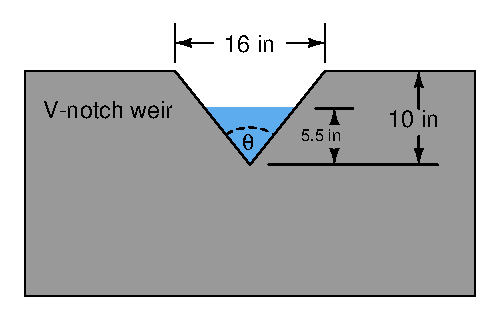
\includegraphics[width=15.5cm]{i00712x01.eps}$$

$$Q = 2.48 \left( \tan {\theta \over 2} \right) H^{2.5} \hbox{\hskip 20pt V-notch weir}$$

\noindent
Der,

$Q$ = Volumetrisk strømningsrate i kubikkfot per sekund (ft$^{3}$/s)

$\theta$ = V-vinkel i grader ($^{o}$)

$H$ = Nivåhode i fot (ft)

\vskip 10pt

Oppgi svaret i CFS, GPM og MCFD (millioner kubikkfot per døgn):

\vskip 10pt

$Q$ = \underbar{\hskip 50pt} CFS

\vskip 10pt

$Q$ = \underbar{\hskip 50pt} GPM

\vskip 10pt

$Q$ = \underbar{\hskip 50pt} MCFD

\underbar{file i00712no}
%(END_QUESTION)





%(BEGIN_ANSWER)

4 poeng for riktig CFS-svar, 3 poeng for hver av de to andre:

\vskip 10pt

$Q$ = \underbar{\bf 0.2822} CFS

\vskip 10pt

$Q$ = \underbar{\bf 126.6} GPM

\vskip 10pt

$Q$ = \underbar{\bf 0.02438} MCFD


%(END_ANSWER)





%(BEGIN_NOTES)

{\bf Denne oppgaven er ment for eksamen, ikke arbeidsark!}.

%(END_NOTES)
